\RequirePackage{lineno}  % http://www-d0.fnal.gov/Run2Physics/WWW/templates/lineno.html
\documentclass[12pt]{iopart}
\newcommand{\gguide}{{\it Preparing graphics for IOP journals}}
%Uncomment next line if AMS fonts required
%\usepackage{iopams}  
% parameters from other files
\newcommand{\citetapos}[1]{\citeauthor{#1}'s \citeyearpar{#1}}  % apostrophe's in cites
%\usepackage[square,numbers,sort&compress]{natbib}
\def\linenumberfont{\normalfont\small\sffamily}
\usepackage{graphicx}
\usepackage{epstopdf}
% From link below: next two lines allow caption to fill the full figure box, and caption formats to be changed (e.g. font)
% http://tex.stackexchange.com/questions/107350/caption-below-the-figure-and-aligned-with-left-side-of-figure
% http://ctan.mackichan.com/macros/latex/contrib/caption/caption-eng.pdf
\usepackage{caption}
\captionsetup[figure]{slc=off, font=footnotesize}
%\usepackage{amsmath}
\usepackage{longtable}
\usepackage{placeins}


\begin{document}
\bibliographystyle{unsrt}

\setpagewiselinenumbers
%\modulolinenumbers[5]
%\linenumbers
\section*{\large Appendix S1: Supplementary Results}
%\begin{table}[ht]
%\centering
%\caption{Confidence classes for the forcing data based on bias-correction weights.}
%\begin{tabular}{cc}
%  \hline
%  Confidence class & Bias-correction weight \\ 
%  \hline
%High & 0.75-1.00 \\ 
%Medium-High & 0.50-0.75\\ 
%Medium-Low & 0.25-0.50\\ 
% Low & 0.05-0.25 \\ 
% None & $<$0.05 \\ 
%   \hline
%\end{tabular}
%\end{table}  
\section*{Landcover map bias}

% latex table generated in R 3.4.1 by xtable 1.8-2 package
% Sun Aug 27 16:09:11 2017
\begin{longtable}{lllrrrrrr}
\caption{Biases and mean absolute errors (MAE) in cropland maps relative to the 2011 reference map for each aggregation scale calculated over the entire country, for the union of agricultural regions (cropland $>$ 0), and as density independent means, wherein the mean bias/MAE values for each of 20 cropland cover classes (representing 5\% increments of cover 0\% to 100\% defined by the reference map) were calculated and then averaged.} \\ 
  \hline
Region & Metric & Map & 1 km & 5 km & 10 km & 25 km & 50 km & 100 km \\ 
  \hline
Country & Bias & SA-LC & -2.5 & -2.5 & -2.5 & -2.5 & -2.5 & -2.5 \\ 
  Country & Bias & GlobCover & 2.0 & 2.0 & 2.0 & 2.0 & 2.0 & 2.0 \\ 
  Country & Bias & MODIS & 2.5 & 2.5 & 2.5 & 2.5 & 2.5 & 2.5 \\ 
  Country & Bias & GLC-Share & -0.6 & -0.6 & -0.6 & -0.6 & -0.6 & -0.6 \\ 
  Country & MAE & SA-LC & 3.3 & 2.9 & 2.8 & 2.7 & 2.6 & 2.6 \\ 
  Country & MAE & GlobCover & 11.3 & 9.4 & 8.8 & 8.2 & 7.6 & 7.2 \\ 
  Country & MAE & MODIS & 7.8 & 6.5 & 6.1 & 5.6 & 5.0 & 4.6 \\ 
  Country & MAE & GLC-Share & 6.3 & 4.5 & 3.9 & 3.2 & 2.6 & 2.2 \\ 
  Agricultural & Bias & SA-LC & -9.1 & -4.3 & -3.3 & -2.9 & -2.7 & -2.6 \\ 
  Agricultural & Bias & GlobCover & 3.7 & 2.8 & 2.5 & 2.2 & 2.1 & 2.1 \\ 
  Agricultural & Bias & MODIS & 7.1 & 4.1 & 3.4 & 2.9 & 2.7 & 2.6 \\ 
  Agricultural & Bias & GLC-Share & -2.0 & -1.0 & -0.8 & -0.6 & -0.6 & -0.6 \\ 
  Agricultural & MAE & SA-LC & 11.1 & 5.0 & 3.7 & 3.0 & 2.8 & 2.6 \\ 
  Agricultural & MAE & GlobCover & 20.5 & 12.8 & 10.7 & 9.0 & 8.1 & 7.3 \\ 
  Agricultural & MAE & MODIS & 22.7 & 10.8 & 8.2 & 6.3 & 5.4 & 4.7 \\ 
  Agricultural & MAE & GLC-Share & 19.2 & 7.8 & 5.3 & 3.7 & 2.9 & 2.2 \\ 
  Density independent & Bias & SA-LC & -8.6 & -7.6 & -7.7 & -7.0 & -6.5 & -5.5 \\ 
  Density independent & Bias & GlobCover & 33.6 & 33.5 & 30.9 & 27.9 & 23.8 & 14.4 \\ 
  Density independent & Bias & MODIS & 20.9 & 13.9 & 11.0 & 8.1 & 7.7 & 7.1 \\ 
  Density independent & Bias & GLC-Share & 4.3 & -1.1 & -1.8 & -2.3 & -0.1 & -0.6 \\ 
  Density independent & MAE & SA-LC & 11.4 & 8.4 & 8.1 & 7.2 & 6.6 & 5.6 \\ 
  Density independent & MAE & GlobCover & 37.1 & 35.8 & 32.9 & 29.7 & 25.9 & 16.9 \\ 
  Density independent & MAE & MODIS & 31.5 & 22.3 & 19.4 & 16.9 & 14.7 & 11.2 \\ 
  Density independent & MAE & GLC-Share & 23.2 & 12.1 & 9.9 & 8.1 & 6.2 & 3.8 \\ 
   \hline
\hline
\end{longtable}


\begin{figure}[ht]
  \centering
     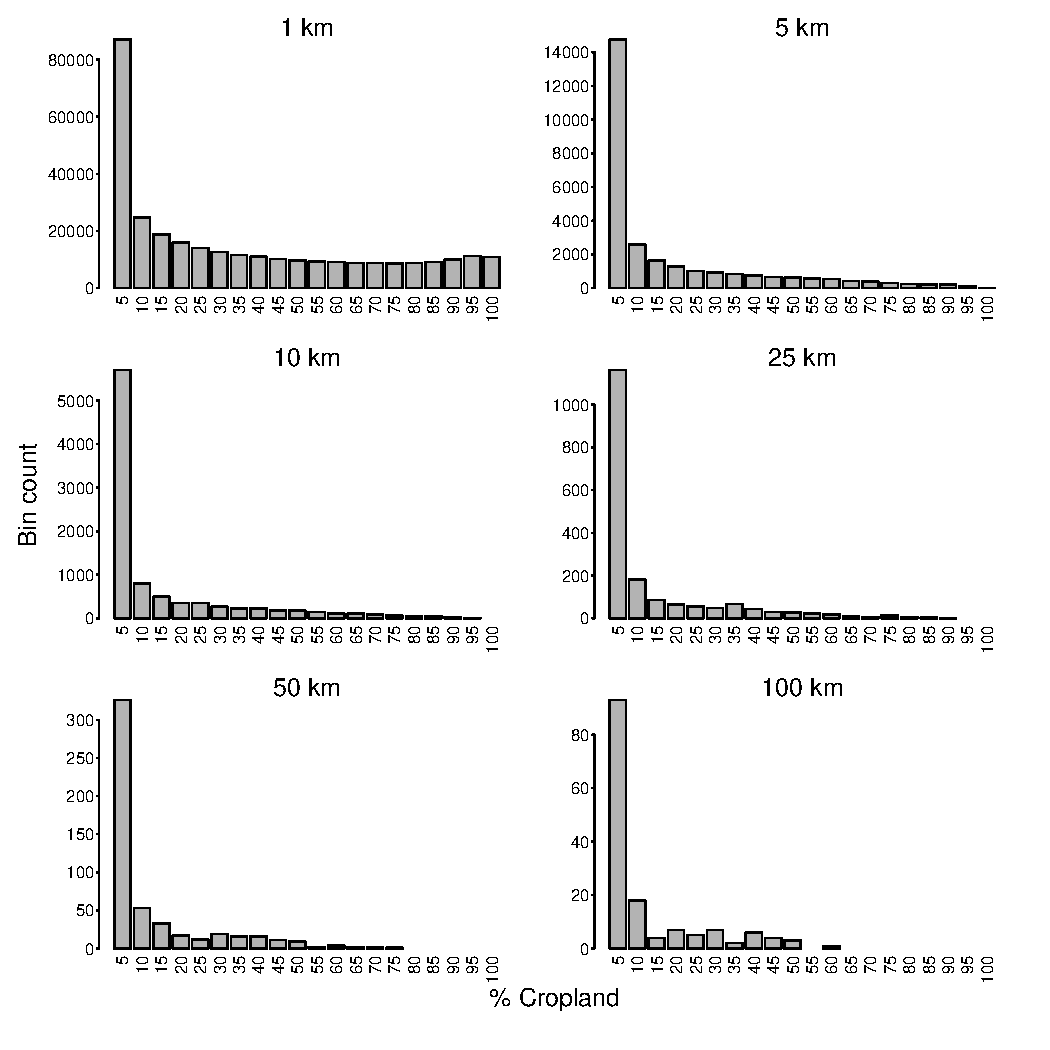
\includegraphics[width = 16cm]{figures/cropland_bins.pdf} 
%     \vspace{-3cm}
      \caption{Number of cells within each cropland density bin at each scale of aggregation, where bins represent 5\% increment of cropland cover from 0 to 100\% (values on x-axis provide the upper limit of each bin).}
      \label{fig:default}
\end{figure}


% latex table generated in R 3.4.1 by xtable 1.8-2 package
% Sun Aug 27 16:11:21 2017
\begin{longtable}{lllrrrrrr}
\caption{Biases and mean absolute errors (MAE) in cropland maps relative to the 2007 reference map for each aggregation scale calculated over the entire country, for the union of agricultural regions, and as density independent means, wherein the mean bias/MAE values for each of 20 cropland cover classes (representing 5\% increments of cover 0\% to 100\% defined by the reference map) were calculated and then averaged.} \\ 
  \hline
Region & Metric & Map & 1 km & 5 km & 10 km & 25 km & 50 km & 100 km \\ 
  \hline
Country & Bias & SA-LC & -2.9 & -2.9 & -2.9 & -2.9 & -2.9 & -2.9 \\ 
  Country & Bias & GlobCover & 1.7 & 1.7 & 1.7 & 1.7 & 1.7 & 1.7 \\ 
  Country & Bias & MODIS & 2.2 & 2.2 & 2.2 & 2.2 & 2.2 & 2.2 \\ 
  Country & Bias & GLC-Share & -0.9 & -0.9 & -0.9 & -0.9 & -0.9 & -0.9 \\ 
  Country & MAE & SA-LC & 3.0 & 2.9 & 2.9 & 2.9 & 2.9 & 2.9 \\ 
  Country & MAE & GlobCover & 11.3 & 9.4 & 8.9 & 8.2 & 7.7 & 7.2 \\ 
  Country & MAE & MODIS & 7.7 & 6.4 & 6.0 & 5.5 & 5.0 & 4.6 \\ 
  Country & MAE & GLC-Share & 6.2 & 4.4 & 3.8 & 3.1 & 2.6 & 2.2 \\ 
  Agricultural & Bias & SA-LC & -9.9 & -4.9 & -3.8 & -3.2 & -3.1 & -2.9 \\ 
  Agricultural & Bias & GlobCover & 3.1 & 2.3 & 2.0 & 1.9 & 1.8 & 1.7 \\ 
  Agricultural & Bias & MODIS & 6.4 & 3.6 & 2.9 & 2.5 & 2.3 & 2.2 \\ 
  Agricultural & Bias & GLC-Share & -2.8 & -1.6 & -1.2 & -1.0 & -1.0 & -0.9 \\ 
  Agricultural & MAE & SA-LC & 10.4 & 5.0 & 3.9 & 3.3 & 3.1 & 3.0 \\ 
  Agricultural & MAE & GlobCover & 20.6 & 12.8 & 10.7 & 9.1 & 8.1 & 7.4 \\ 
  Agricultural & MAE & MODIS & 22.6 & 10.6 & 8.0 & 6.2 & 5.3 & 4.7 \\ 
  Agricultural & MAE & GLC-Share & 19.2 & 7.7 & 5.2 & 3.6 & 2.8 & 2.2 \\ 
  Density independent & Bias & SA-LC & -9.9 & -8.5 & -8.4 & -7.4 & -6.9 & -6.6 \\ 
  Density independent & Bias & GlobCover & 33.8 & 33.8 & 31.2 & 27.4 & 21.6 & 14.8 \\ 
  Density independent & Bias & MODIS & 20.8 & 13.3 & 10.5 & 7.0 & 6.9 & 7.0 \\ 
  Density independent & Bias & GLC-Share & 3.8 & -1.8 & -2.5 & -2.8 & -0.8 & -1.5 \\ 
  Density independent & MAE & SA-LC & 10.5 & 8.6 & 8.4 & 7.4 & 6.9 & 6.6 \\ 
  Density independent & MAE & GlobCover & 37.4 & 36.1 & 33.2 & 29.3 & 24.0 & 17.4 \\ 
  Density independent & MAE & MODIS & 31.7 & 22.2 & 19.5 & 17.2 & 14.5 & 11.6 \\ 
  Density independent & MAE & GLC-Share & 23.3 & 12.0 & 9.8 & 8.2 & 5.9 & 3.9 \\ 
   \hline
\hline
\end{longtable}



\begin{figure}[ht]
  \centering
     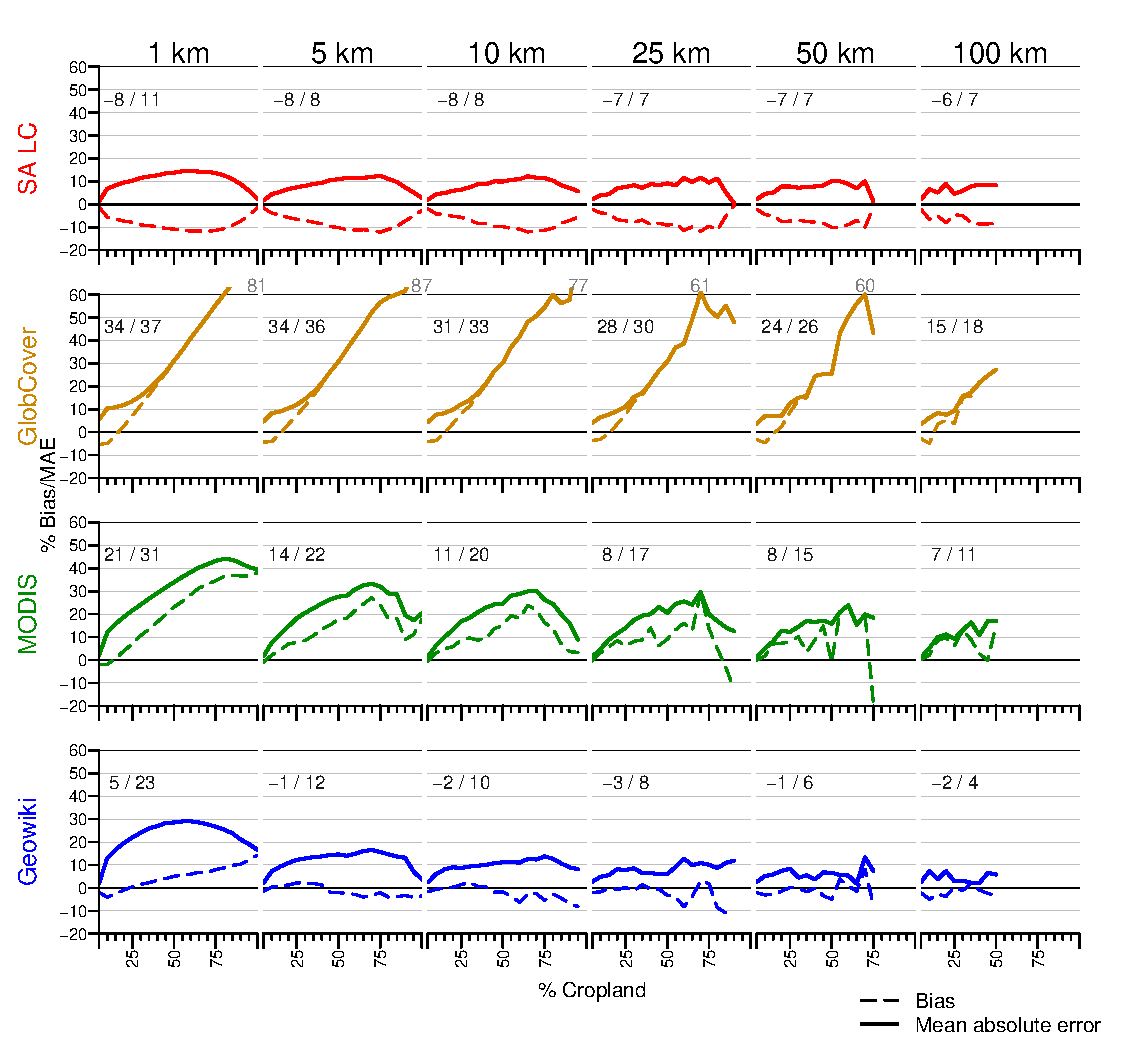
\includegraphics[width = 16cm]{figures/biases_1-100km.pdf} 
%     \vspace{-3cm}
      \caption{Biases and mean absolute errors (MAE) for each of the cropland maps as a function of cropland density (calculated using the 2011 reference maps) and aggregation scales. Rows present biases by map product, columns by aggregation scale.  Dash lines indicate bias at each level of cropland density, calculated in bins spanning 5\% of density (e.g. 0-5\% cropland cover, 5-10\%, etc.), while solid lines indicate the mean absolute error.  The black numbers in each plot area present the overall means of bias/MAE for each sensor-scale combination. The bin-wise and overall mean statistics were calculated from pooled map errors calculated from differences between the 2007 reference map and each cropland map (including all three variants--high, medium, and low--of the MODIS and GlobCover-derived cropland maps), and the 2011 reference map and each cropland map. }
      \label{fig:default}
\end{figure}

%\vspace{0.5 cm}
%\begin{equation}
%\hspace*{1.5 cm} 
%   \label{metric}
%     R_n  = \frac{(1 - \alpha)dswr + dlwr - \sigma * T^4}{\lambda}
%\end{equation}

\begin{figure}[ht]
  \centering
     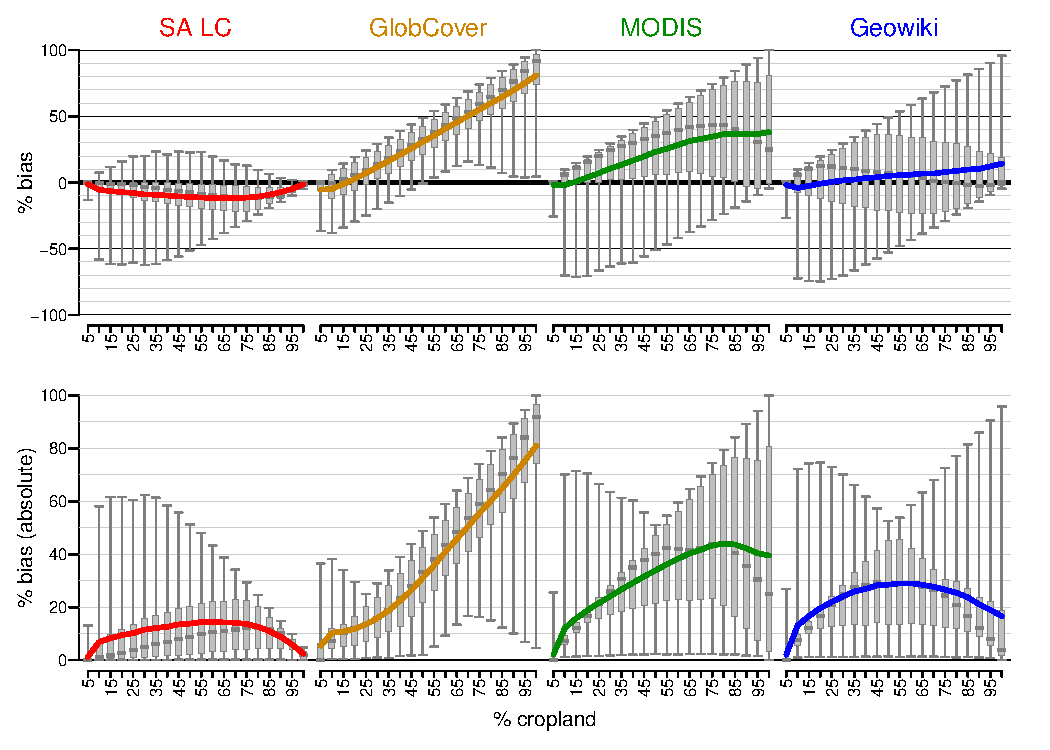
\includegraphics[width = 12cm]{figures/biases_1km.pdf} 
%     \vspace{-3cm}
      \caption{Biases and mean absolute errors (MAE) for each of the cropland maps at 1 km resolution, as a function of cropland density. Colored lines (color-coded to map product name) show the bias/MAE at each level of cropland density, calculated in bins spanning 5\% (e.g. 0-5\% cropland cover, 5-10\%, etc.). Box plots show the variability of bias in each bin (whiskers = 2.5 and 97.5 percentiles, box the inter-quartile, and grey bar in box the median). Biases are presented in the top row, and MAEs in the bottom row. Statistics were calculated from pooled map errors calculated from differences between the 2007 reference map and each cropland map (including all three variants--high, medium, and low--of the MODIS and GlobCover-derived cropland maps), and the 2011 reference map and each cropland map. }
      \label{fig:default}
\end{figure}

\begin{figure}[ht]
  \centering
     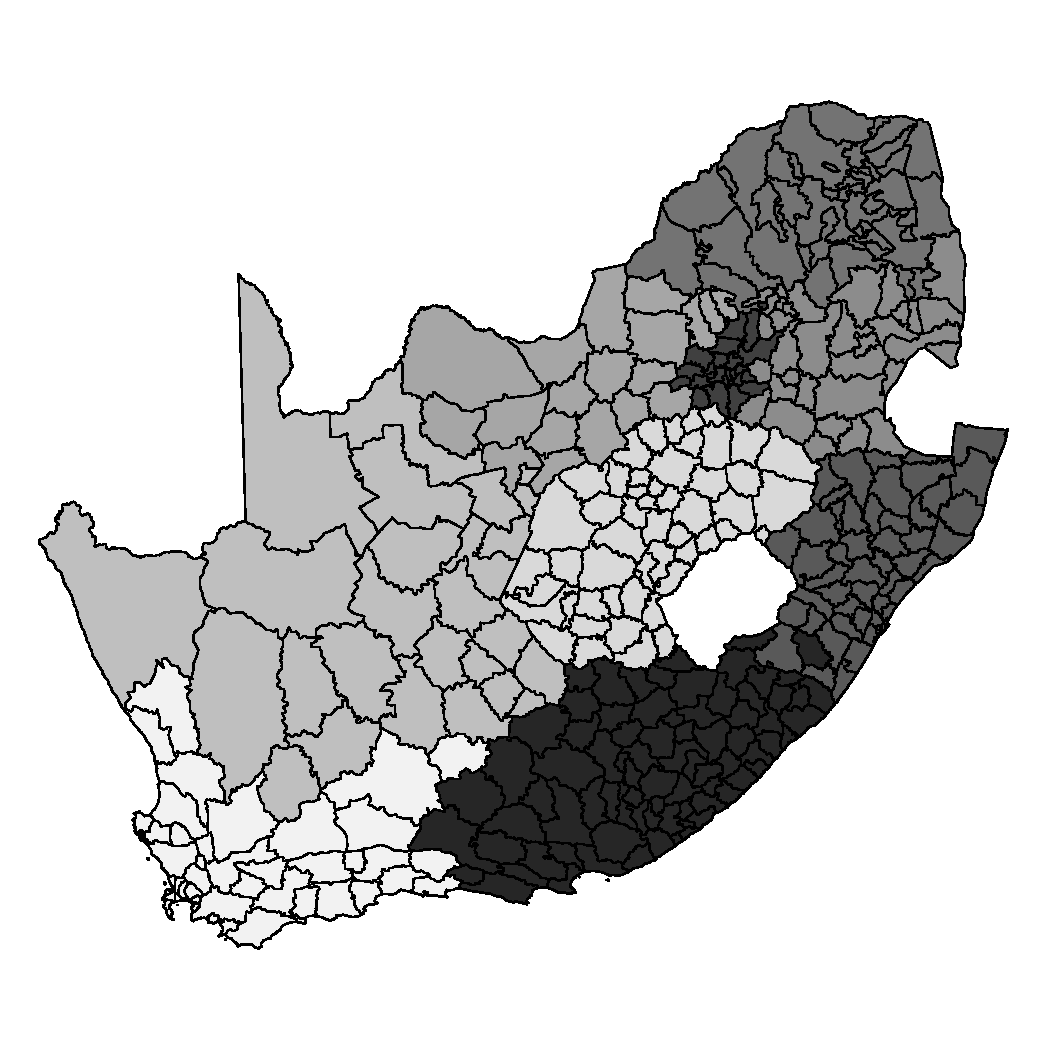
\includegraphics[width = 8cm]{figures/md_map.pdf} 
%     \vspace{-3cm}
      \caption{South Africa's magisterial districts.}
      \label{fig:default}
\end{figure}

\FloatBarrier
\section*{Carbon bias}
\begin{figure}[ht]
  \centering
     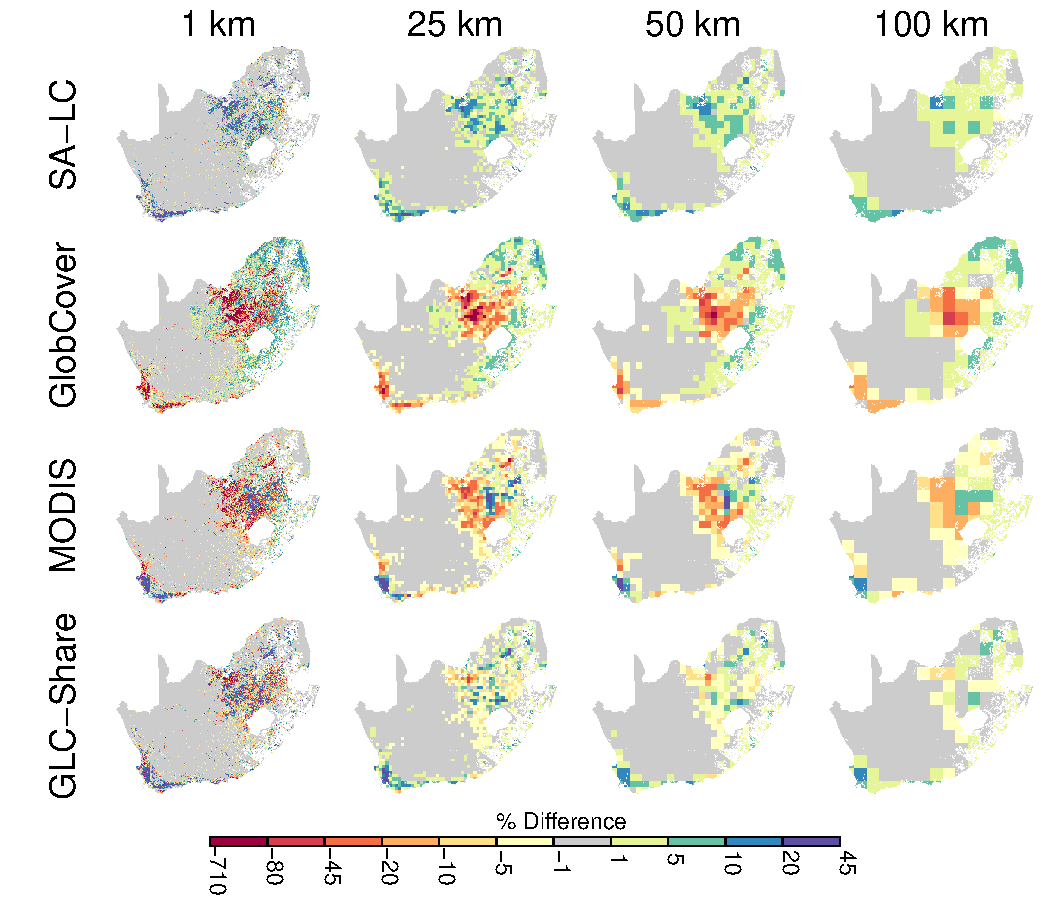
\includegraphics[width = 12cm]{figures/carbon_bias_map.pdf} 
%     \vspace{-3cm}
      \caption{Spatial patterns of error (averaged across four different possible cover types adjacent to cropland) in carbon stock estimates. }
      \label{fig:default}
\end{figure}

% latex table generated in R 3.2.1 by xtable 1.7-4 package
% Fri Oct 16 23:40:37 2015
\begin{table}[ht]
\centering
\caption{Percent differences in total carbon stock estimates calculated from the reference maps and from each of the four cropland maps. Differences are evaluated for total carbon estimates either at the country scale or over just the agricultural regions (cropland $>$0.05\%), using the carbon densities of 5 different cover types to provide the values for the non-agricultural portions of each pixel (cover types indicated by column names).} 
\begin{tabular}{llrrrrr}
  \hline
Region & Map & Forest & Secondary & Shrubland & Grassland & Sparse \\ 
  \hline
Country & SA-LC & 2.6 & 2.5 & 2.5 & 0.1 & -2.1 \\ 
  Country & GlobCover & -2.1 & -2.0 & -2.0 & -0.1 & 1.7 \\ 
  Country & MODIS & -2.6 & -2.5 & -2.5 & -0.1 & 2.1 \\ 
  Country & GeoWiki & 0.6 & 0.5 & 0.5 & 0.0 & -0.5 \\ 
  Agricultural & SA-LC & -2.0 & -2.7 & -2.8 & -10.6 & -14.9 \\ 
  Agricultural & GlobCover & -161.9 & -156.3 & -155.5 & -95.9 & -63.6 \\ 
  Agricultural & MODIS & -1.6 & -0.8 & -0.7 & 8.4 & 13.3 \\ 
  Agricultural & GeoWiki & 7.7 & 7.3 & 7.2 & 2.9 & 0.5 \\ 
   \hline
\end{tabular}
\end{table}


\FloatBarrier
% latex table generated in R 3.2.1 by xtable 1.7-4 package
% Thu Oct  1 15:30:34 2015
\begin{longtable}{lllrrrrrr}
\caption{Biases and mean absolute errors for each of the cropland maps across aggregation scales and each possible landcover type sharing the pixel with cropland. Metrics were calculated across the union of agricultural areas (cropland $>$0.05\%) identified by the reference map and the cropland map to which it was being compared} \\ 
  \hline
Metric & Cover & Map & 1 km & 5 km & 10 km & 25 km & 50 km & 100 km \\ 
  \hline
Bias & All & GeoWiki & -5.6 & 0.8 & 0.8 & 0.5 & 0.4 & 0.4 \\ 
  Bias & All & GlobCover & -23.9 & -8.5 & -6.5 & -4.7 & -3.6 & -2.7 \\ 
  Bias & All & MODIS & -22.1 & -5.3 & -3.9 & -2.9 & -2.4 & -1.9 \\ 
  Bias & All & SA-LC & 7.2 & 4.0 & 3.2 & 2.6 & 2.2 & 1.9 \\ 
  Bias & Forest & GeoWiki & -11.9 & 1.9 & 1.7 & 1.2 & 0.9 & 0.8 \\ 
  Bias & Forest & GlobCover & -51.9 & -16.6 & -12.5 & -9.0 & -6.9 & -5.3 \\ 
  Bias & Forest & MODIS & -47.8 & -10.9 & -7.9 & -6.0 & -5.1 & -4.2 \\ 
  Bias & Forest & SA-LC & 15.6 & 8.6 & 7.0 & 5.5 & 4.8 & 4.2 \\ 
  Bias & Grassland & GeoWiki & 0.1 & 0.1 & 0.0 & 0.0 & 0.0 & 0.0 \\ 
  Bias & Grassland & GlobCover & -0.2 & -0.1 & -0.1 & -0.1 & -0.1 & -0.1 \\ 
  Bias & Grassland & MODIS & -0.3 & -0.2 & -0.2 & -0.1 & -0.1 & -0.1 \\ 
  Bias & Grassland & SA-LC & 0.3 & 0.2 & 0.2 & 0.1 & 0.1 & 0.1 \\ 
  Bias & Secondary & GeoWiki & -6.9 & 1.6 & 1.5 & 1.1 & 0.8 & 0.8 \\ 
  Bias & Secondary & GlobCover & -34.2 & -13.2 & -10.3 & -7.8 & -6.1 & -4.7 \\ 
  Bias & Secondary & MODIS & -33.3 & -9.4 & -7.0 & -5.5 & -4.7 & -3.9 \\ 
  Bias & Secondary & SA-LC & 13.5 & 7.6 & 6.2 & 5.0 & 4.4 & 3.9 \\ 
  Bias & Shrubland & GeoWiki & -6.5 & 1.6 & 1.4 & 1.1 & 0.8 & 0.8 \\ 
  Bias & Shrubland & GlobCover & -32.6 & -12.8 & -10.0 & -7.6 & -6.0 & -4.7 \\ 
  Bias & Shrubland & MODIS & -31.9 & -9.2 & -6.9 & -5.4 & -4.7 & -3.9 \\ 
  Bias & Shrubland & SA-LC & 13.2 & 7.5 & 6.1 & 5.0 & 4.4 & 3.8 \\ 
  Bias & Sparse & GeoWiki & -2.8 & -1.0 & -0.8 & -0.8 & -0.7 & -0.6 \\ 
  Bias & Sparse & GlobCover & -0.7 & 0.4 & 0.6 & 0.9 & 1.0 & 1.1 \\ 
  Bias & Sparse & MODIS & 2.9 & 2.9 & 2.8 & 2.7 & 2.6 & 2.5 \\ 
  Bias & Sparse & SA-LC & -6.7 & -3.8 & -3.3 & -2.9 & -2.8 & -2.5 \\ 
  MAE & All & GeoWiki & 26.8 & 9.4 & 6.5 & 4.5 & 3.4 & 2.4 \\ 
  MAE & All & GlobCover & 36.7 & 17.0 & 14.0 & 11.5 & 9.6 & 8.0 \\ 
  MAE & All & MODIS & 37.8 & 13.8 & 10.8 & 8.4 & 6.7 & 5.5 \\ 
  MAE & All & SA-LC & 13.6 & 6.3 & 4.9 & 3.9 & 3.4 & 3.0 \\ 
  MAE & Forest & GeoWiki & 45.9 & 14.3 & 9.8 & 6.6 & 4.8 & 3.4 \\ 
  MAE & Forest & GlobCover & 68.8 & 27.5 & 22.0 & 17.4 & 14.2 & 11.6 \\ 
  MAE & Forest & MODIS & 69.1 & 21.7 & 16.6 & 12.6 & 9.9 & 7.9 \\ 
  MAE & Forest & SA-LC & 22.1 & 9.6 & 7.5 & 5.8 & 4.9 & 4.3 \\ 
  MAE & Grassland & GeoWiki & 0.8 & 0.3 & 0.3 & 0.2 & 0.1 & 0.1 \\ 
  MAE & Grassland & GlobCover & 0.8 & 0.6 & 0.5 & 0.4 & 0.4 & 0.3 \\ 
  MAE & Grassland & MODIS & 0.9 & 0.5 & 0.4 & 0.3 & 0.3 & 0.2 \\ 
  MAE & Grassland & SA-LC & 0.5 & 0.2 & 0.2 & 0.2 & 0.1 & 0.1 \\ 
  MAE & Secondary & GeoWiki & 36.8 & 12.8 & 8.8 & 6.0 & 4.4 & 3.2 \\ 
  MAE & Secondary & GlobCover & 50.2 & 23.5 & 19.3 & 15.6 & 13.0 & 10.7 \\ 
  MAE & Secondary & MODIS & 52.3 & 19.1 & 14.9 & 11.4 & 9.1 & 7.3 \\ 
  MAE & Secondary & SA-LC & 18.7 & 8.6 & 6.7 & 5.3 & 4.5 & 4.0 \\ 
  MAE & Shrubland & GeoWiki & 35.8 & 12.6 & 8.7 & 6.0 & 4.4 & 3.2 \\ 
  MAE & Shrubland & GlobCover & 48.5 & 23.0 & 19.0 & 15.4 & 12.8 & 10.6 \\ 
  MAE & Shrubland & MODIS & 50.7 & 18.8 & 14.7 & 11.3 & 9.0 & 7.2 \\ 
  MAE & Shrubland & SA-LC & 18.3 & 8.4 & 6.6 & 5.2 & 4.5 & 3.9 \\ 
  MAE & Sparse & GeoWiki & 14.7 & 6.9 & 5.2 & 3.8 & 3.0 & 2.3 \\ 
  MAE & Sparse & GlobCover & 15.3 & 10.5 & 9.4 & 8.5 & 7.7 & 6.8 \\ 
  MAE & Sparse & MODIS & 16.2 & 9.0 & 7.6 & 6.3 & 5.4 & 4.6 \\ 
  MAE & Sparse & SA-LC & 8.6 & 4.4 & 3.7 & 3.1 & 2.9 & 2.6 \\ 
   \hline
\hline
\end{longtable}


% latex table generated in R 3.2.1 by xtable 1.7-4 package
% Thu Sep 24 06:16:07 2015
\begin{longtable}{lllrrrrrr}
\caption{Biases and mean absolute errors for each of the cropland maps across aggregation scales and each possible landcover type sharing the pixel with cropland. Means were calculated across the entire country.} \\ 
  \hline
Metric & Map & Cover & 1 km & 5 km & 10 km & 25 km & 50 km & 100 km \\ 
  \hline
Bias & GeoWiki & All & -1.7 & 0.4 & 0.4 & 0.3 & 0.2 & 0.3 \\ 
  Bias & GlobCover & All & -12.6 & -5.6 & -4.5 & -3.4 & -2.7 & -2.2 \\ 
  Bias & MODIS & All & -7.3 & -2.8 & -2.3 & -1.9 & -1.7 & -1.5 \\ 
  Bias & SA-LC & All & 2.1 & 2.0 & 1.8 & 1.7 & 1.5 & 1.5 \\ 
  Bias & GeoWiki & Forest & -3.7 & 0.9 & 0.9 & 0.8 & 0.6 & 0.6 \\ 
  Bias & GlobCover & Forest & -27.3 & -10.9 & -8.7 & -6.5 & -5.2 & -4.3 \\ 
  Bias & MODIS & Forest & -15.8 & -5.7 & -4.6 & -4.0 & -3.6 & -3.2 \\ 
  Bias & SA-LC & Forest & 4.5 & 4.2 & 3.9 & 3.6 & 3.4 & 3.2 \\ 
  Bias & GeoWiki & Grassland & 0.0 & 0.0 & 0.0 & 0.0 & 0.0 & 0.0 \\ 
  Bias & GlobCover & Grassland & -0.1 & -0.1 & -0.1 & -0.1 & -0.1 & -0.1 \\ 
  Bias & MODIS & Grassland & -0.1 & -0.1 & -0.1 & -0.1 & -0.1 & -0.1 \\ 
  Bias & SA-LC & Grassland & 0.1 & 0.1 & 0.1 & 0.1 & 0.1 & 0.1 \\ 
  Bias & GeoWiki & Secondary & -2.1 & 0.8 & 0.8 & 0.7 & 0.6 & 0.6 \\ 
  Bias & GlobCover & Secondary & -18.0 & -8.7 & -7.1 & -5.6 & -4.6 & -3.8 \\ 
  Bias & MODIS & Secondary & -11.0 & -4.9 & -4.1 & -3.6 & -3.3 & -3.0 \\ 
  Bias & SA-LC & Secondary & 3.9 & 3.7 & 3.5 & 3.3 & 3.1 & 3.0 \\ 
  Bias & GeoWiki & Shrubland & -2.0 & 0.8 & 0.8 & 0.7 & 0.5 & 0.6 \\ 
  Bias & GlobCover & Shrubland & -17.1 & -8.4 & -7.0 & -5.5 & -4.5 & -3.8 \\ 
  Bias & MODIS & Shrubland & -10.6 & -4.8 & -4.1 & -3.5 & -3.2 & -2.9 \\ 
  Bias & SA-LC & Shrubland & 3.8 & 3.6 & 3.5 & 3.2 & 3.0 & 2.9 \\ 
  Bias & GeoWiki & Sparse & -0.9 & -0.5 & -0.5 & -0.5 & -0.5 & -0.5 \\ 
  Bias & GlobCover & Sparse & -0.4 & 0.3 & 0.4 & 0.6 & 0.8 & 0.9 \\ 
  Bias & MODIS & Sparse & 0.9 & 1.5 & 1.6 & 1.8 & 1.8 & 1.9 \\ 
  Bias & SA-LC & Sparse & -1.9 & -1.9 & -1.9 & -1.9 & -1.9 & -1.9 \\ 
  MAE & GeoWiki & All & 8.3 & 4.6 & 3.7 & 3.0 & 2.3 & 1.9 \\ 
  MAE & GlobCover & All & 19.3 & 11.2 & 9.8 & 8.3 & 7.2 & 6.5 \\ 
  MAE & MODIS & All & 12.5 & 7.2 & 6.4 & 5.5 & 4.7 & 4.1 \\ 
  MAE & SA-LC & All & 3.9 & 3.1 & 2.8 & 2.5 & 2.4 & 2.3 \\ 
  MAE & GeoWiki & Forest & 14.3 & 7.0 & 5.6 & 4.3 & 3.3 & 2.6 \\ 
  MAE & GlobCover & Forest & 36.2 & 18.1 & 15.3 & 12.6 & 10.7 & 9.3 \\ 
  MAE & MODIS & Forest & 22.9 & 11.4 & 9.8 & 8.2 & 6.8 & 5.9 \\ 
  MAE & SA-LC & Forest & 6.3 & 4.7 & 4.2 & 3.8 & 3.5 & 3.3 \\ 
  MAE & GeoWiki & Grassland & 0.2 & 0.2 & 0.1 & 0.1 & 0.1 & 0.1 \\ 
  MAE & GlobCover & Grassland & 0.4 & 0.4 & 0.3 & 0.3 & 0.3 & 0.3 \\ 
  MAE & MODIS & Grassland & 0.3 & 0.2 & 0.2 & 0.2 & 0.2 & 0.2 \\ 
  MAE & SA-LC & Grassland & 0.1 & 0.1 & 0.1 & 0.1 & 0.1 & 0.1 \\ 
  MAE & GeoWiki & Secondary & 11.5 & 6.3 & 5.0 & 3.9 & 3.1 & 2.4 \\ 
  MAE & GlobCover & Secondary & 26.4 & 15.5 & 13.4 & 11.3 & 9.8 & 8.6 \\ 
  MAE & MODIS & Secondary & 17.3 & 10.0 & 8.7 & 7.4 & 6.3 & 5.5 \\ 
  MAE & SA-LC & Secondary & 5.3 & 4.2 & 3.8 & 3.5 & 3.2 & 3.0 \\ 
  MAE & GeoWiki & Shrubland & 11.2 & 6.2 & 5.0 & 3.9 & 3.0 & 2.4 \\ 
  MAE & GlobCover & Shrubland & 25.5 & 15.2 & 13.2 & 11.1 & 9.6 & 8.5 \\ 
  MAE & MODIS & Shrubland & 16.8 & 9.8 & 8.6 & 7.3 & 6.2 & 5.4 \\ 
  MAE & SA-LC & Shrubland & 5.2 & 4.1 & 3.8 & 3.4 & 3.1 & 3.0 \\ 
  MAE & GeoWiki & Sparse & 4.6 & 3.4 & 3.0 & 2.5 & 2.1 & 1.7 \\ 
  MAE & GlobCover & Sparse & 8.0 & 6.9 & 6.6 & 6.2 & 5.8 & 5.5 \\ 
  MAE & MODIS & Sparse & 5.4 & 4.7 & 4.5 & 4.1 & 3.8 & 3.5 \\ 
  MAE & SA-LC & Sparse & 2.5 & 2.2 & 2.1 & 2.0 & 2.0 & 2.0 \\ 
   \hline
\hline
\end{longtable}



\section*{Yield and Harvested Area Bias}
\begin{figure}[ht]
  \centering
     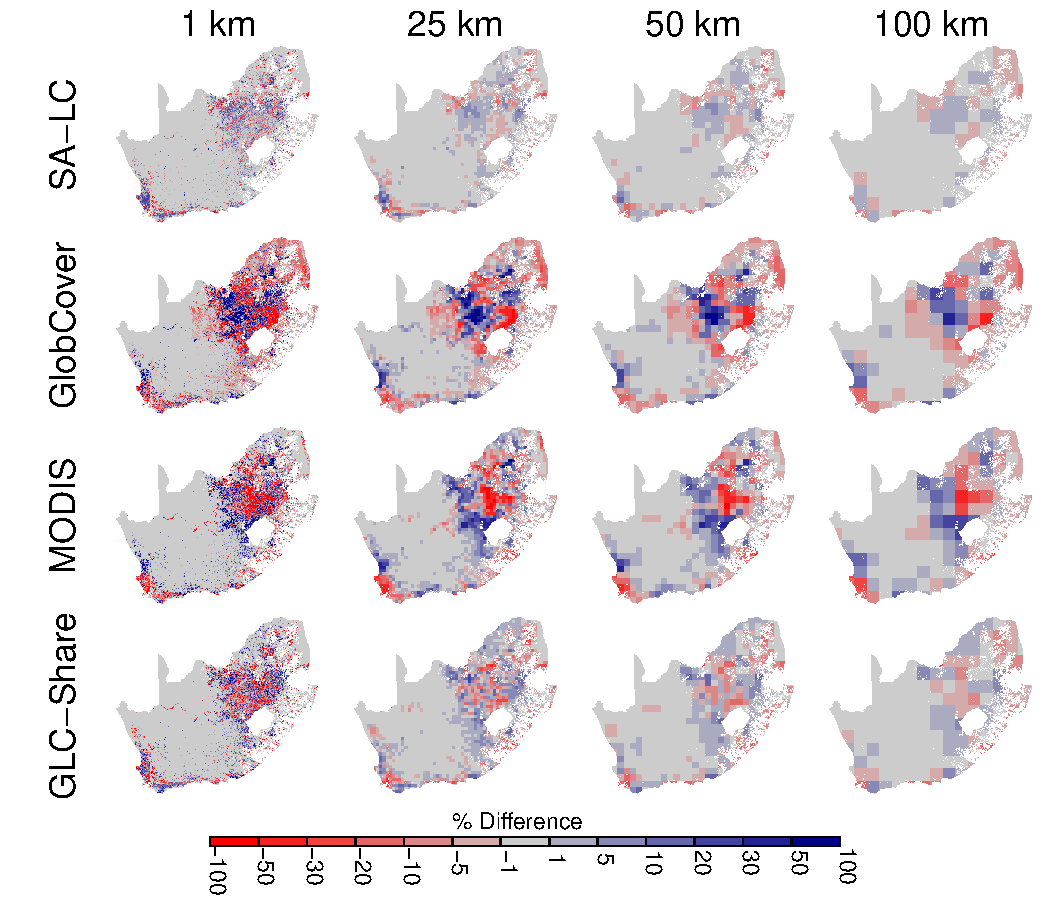
\includegraphics[width = 12cm]{figures/cropland_adj_bias_map2.pdf} 
      \caption{Errors in cropland maps adjusted using provincial cropland area statistics.}
      \label{fig:default}
\end{figure}

\FloatBarrier
\input{figures/cropadj-mae.tex}

\clearpage
\begin{figure}[ht]
  \centering
     \includegraphics[width = 12cm]{figures/yld_bias_map_1.pdf} 
      \caption{Errors (normalized to the reference-derived country mean) in disaggregated maize yield estimates.}
      \label{fig:default}
\end{figure}

\begin{figure}[ht]
  \centering
     \includegraphics[width = 12cm]{figures/prod_bias_map_1.pdf} 
      \caption{Errors (normalized to reference-derived country mean) production estimates calculated from disaggregated maize yield and harvested area estimates.}
      \label{fig:default}
\end{figure}

\FloatBarrier
% latex table generated in R 3.4.1 by xtable 1.8-2 package
% Fri Sep  1 15:01:36 2017
\begin{longtable}{llllrrrrrr}
\caption{Biases and mean absolute errors (MAE) in disaggregated maize yield and production (calculated from disaggregated yield and harvested area estimates) maps. Values for both density-weighted and agricultural areas bias and accuracy are presennted. Bias and MAE were normalized to their respective mean values calculated from reference maps.} \\ 
  \hline
Region & Metric & Map & Variable & 1 km & 5 km & 10 km & 25 km & 50 km & 100 km \\ 
  \hline
Density & Bias & SA-LC & Yield & 1.2 & 0.3 & 0.0 & 0.0 & 0.0 & -0.3 \\ 
  Density & Bias & GlobCover & Yield & 9.8 & 0.9 & 0.0 & -0.6 & -0.6 & -0.6 \\ 
  Density & Bias & MODIS & Yield & 19.6 & 8.9 & 5.7 & 3.0 & 1.5 & -0.6 \\ 
  Density & Bias & GLC-Share & Yield & 8.0 & 3.0 & 1.5 & 0.6 & 0.3 & -0.6 \\ 
  Density & Bias & SA-LC & Production & 6.9 & 1.6 & 0.5 & -0.2 & -0.1 & -0.1 \\ 
  Density & Bias & GlobCover & Production & 60.5 & 50.2 & 43.7 & 35.1 & 23.3 & 12.5 \\ 
  Density & Bias & MODIS & Production & 21.9 & 6.0 & 1.8 & -1.8 & -0.9 & -0.5 \\ 
  Density & Bias & GLC-Share & Production & 12.7 & -3.3 & -4.6 & -3.8 & -0.5 & -0.9 \\ 
  Density & MAE & SA-LC & Yield & 1.2 & 0.3 & 0.3 & 0.3 & 0.6 & 0.9 \\ 
  Density & MAE & GlobCover & Yield & 9.8 & 1.2 & 0.9 & 1.5 & 1.8 & 1.8 \\ 
  Density & MAE & MODIS & Yield & 19.6 & 9.2 & 6.2 & 4.5 & 3.9 & 2.4 \\ 
  Density & MAE & GLC-Share & Yield & 8.0 & 3.3 & 1.8 & 1.8 & 1.2 & 1.2 \\ 
  Density & MAE & SA-LC & Production & 19.0 & 14.3 & 11.8 & 8.9 & 5.1 & 2.3 \\ 
  Density & MAE & GlobCover & Production & 95.6 & 102.0 & 100.4 & 88.1 & 65.8 & 46.4 \\ 
  Density & MAE & MODIS & Production & 66.8 & 62.0 & 58.4 & 46.4 & 25.7 & 14.6 \\ 
  Density & MAE & GLC-Share & Production & 47.3 & 43.6 & 37.6 & 29.3 & 19.4 & 7.9 \\ 
  Agricultural & Bias & SA-LC & Yield & -5.1 & -0.3 & 3.0 & 3.6 & 3.6 & 1.5 \\ 
  Agricultural & Bias & GlobCover & Yield & -58.0 & -36.0 & -22.3 & -11.9 & -8.9 & -1.5 \\ 
  Agricultural & Bias & MODIS & Yield & 5.1 & 21.4 & 29.2 & 26.8 & 20.5 & 11.6 \\ 
  Agricultural & Bias & GLC-Share & Yield & 2.4 & 24.4 & 29.5 & 25.3 & 21.4 & 9.8 \\ 
  Agricultural & Bias & SA-LC & Production & 0.0 & -0.1 & -0.1 & -0.1 & -0.0 & 0.0 \\ 
  Agricultural & Bias & GlobCover & Production & 0.0 & -0.1 & 0.0 & 0.1 & 0.3 & 0.3 \\ 
  Agricultural & Bias & MODIS & Production & 0.0 & -0.1 & -0.1 & -0.1 & 0.0 & -0.1 \\ 
  Agricultural & Bias & GLC-Share & Production & 0.0 & 0.1 & 0.0 & 0.0 & 0.1 & 0.1 \\ 
  Agricultural & MAE & SA-LC & Yield & 15.5 & 16.7 & 19.9 & 15.8 & 12.2 & 6.8 \\ 
  Agricultural & MAE & GlobCover & Yield & 71.7 & 48.2 & 38.1 & 23.5 & 17.3 & 6.2 \\ 
  Agricultural & MAE & MODIS & Yield & 55.9 & 51.2 & 50.9 & 44.9 & 38.4 & 20.8 \\ 
  Agricultural & MAE & GLC-Share & Yield & 41.1 & 41.1 & 40.5 & 35.1 & 28.6 & 14.6 \\ 
  Agricultural & MAE & SA-LC & Production & 19.7 & 11.3 & 8.6 & 5.5 & 3.3 & 1.9 \\ 
  Agricultural & MAE & GlobCover & Production & 55.7 & 55.5 & 52.5 & 42.2 & 28.1 & 17.3 \\ 
  Agricultural & MAE & MODIS & Production & 56.0 & 41.3 & 35.6 & 24.9 & 14.1 & 8.4 \\ 
  Agricultural & MAE & GLC-Share & Production & 43.7 & 30.2 & 23.5 & 15.3 & 9.3 & 4.0 \\ 
   \hline
\hline
\end{longtable}


\section*{Evapotranspiration bias}
% latex table generated in R 3.2.1 by xtable 1.7-4 package
% Thu Sep 24 11:01:34 2015
\begin{longtable}{llrr}
\caption{Biases and mean absolute errors (as \%) for evapotranspiration variables derived from a 29-year time series calculated by the VIC model, including the average total ET for the 3 months of the year when ET is highest, the annual mean and the minimum and maximum annual ETs in the time series.} \\ 
  \hline
Variable & Map & Bias & Abs Bias \\ 
  \hline
Peak & GeoWiki & 0.2 & 0.8 \\ 
  Annual Mean & GeoWiki & 0.3 & 0.7 \\ 
  29-year Min & GeoWiki & 0.3 & 0.6 \\ 
  29-year Max & GeoWiki & 0.3 & 0.8 \\ 
  Peak & GlobCover & 0.1 & 1.2 \\ 
  Annual Mean & GlobCover & -0.1 & 1.0 \\ 
  29-year Min & GlobCover & -0.2 & 0.9 \\ 
  29-year Max & GlobCover & 0.2 & 1.2 \\ 
  Peak & MODIS & -0.5 & 0.9 \\ 
  Annual Mean & MODIS & -0.6 & 0.8 \\ 
  29-year Min & MODIS & -0.6 & 0.7 \\ 
  29-year Max & MODIS & -0.5 & 0.8 \\ 
  Peak & SA-LC & 0.3 & 0.7 \\ 
  Annual Mean & SA-LC & 0.5 & 0.6 \\ 
  29-year Min & SA-LC & 0.4 & 0.5 \\ 
  29-year Max & SA-LC & 0.4 & 0.6 \\ 
   \hline
\hline
\end{longtable}


\section*{Agent allocation bias}

\begin{figure}[ht]
  \centering
     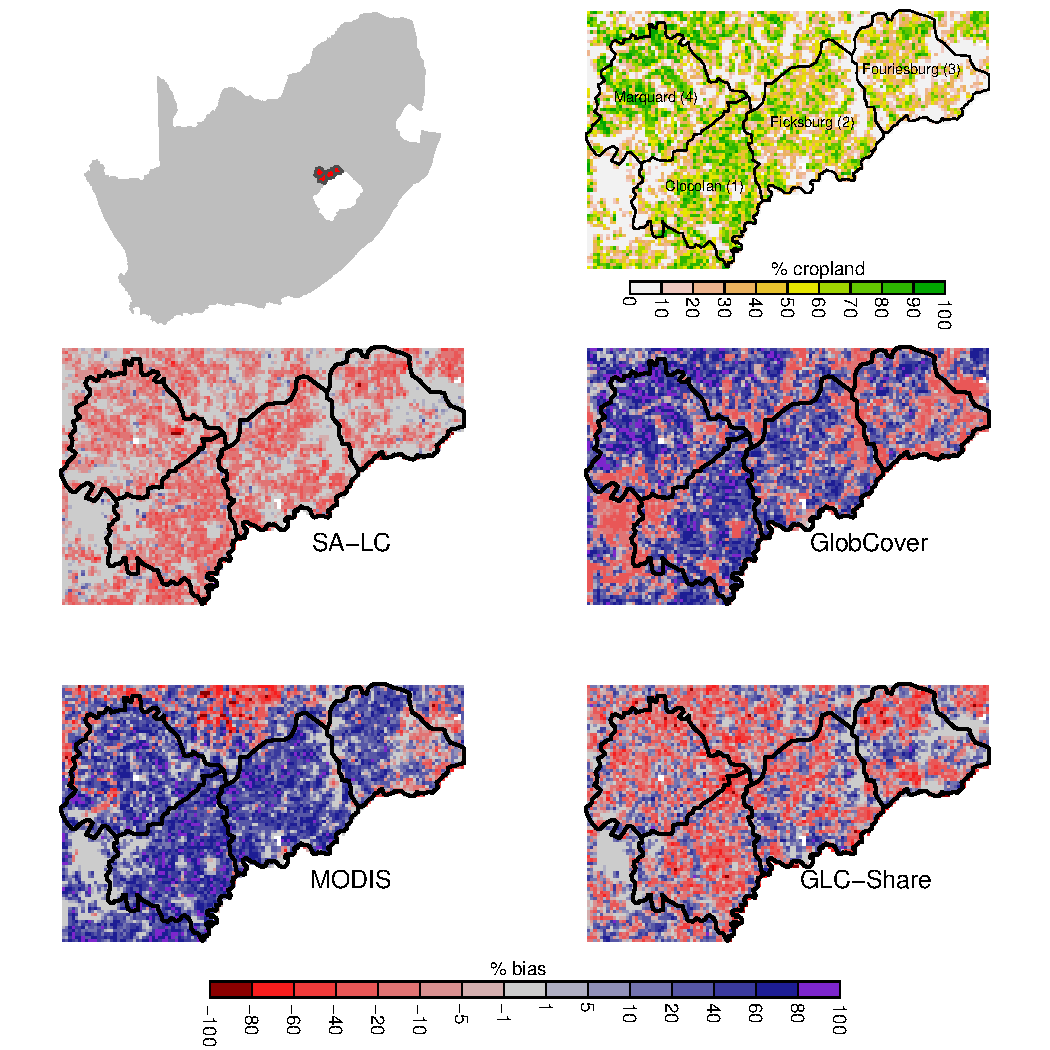
\includegraphics[width = 12cm]{figures/abm-selected-districts.pdf} 
      \caption{The location of the four selected magisterial districts (top left) used in evaluating agent allocation bias, the reference levels of cropland cover within those districts (top right), and the difference in cropland percentage between the reference and each of the four cropland maps (lower four panels). }
      \label{fig:default}
\end{figure}



\FloatBarrier
\section*{References}
\bibliography{}
\end{document}  

